\documentclass[journal,transmag]{IEEEtran}

\usepackage[pdftex]{graphicx}
\usepackage{amsmath}
\usepackage[algoruled, noend]{algorithm2e}
\usepackage{array}
\usepackage{subcaption}
\usepackage{url}

\begin{document}

\newcommand{\lo}{\left(}
\newcommand{\ro}{\right)} 
\newcommand{\bs}[1]{\textit{\textbf{#1}}}
\newcommand{\bsm}[1]{\boldsymbol{#1}}
\newcommand{\pds}[2]{\frac{\partial{#1}}{\partial{#2}}}
\newcommand{\pdv}[2]{\frac{\partial{#1}}{\partial{\bs{#2}}}}
\renewcommand{\d}[2]{\frac{d{#1}}{d{#2}}}
\newcommand{\mc}[1]{\mathcal{#1}}
\newcommand{\phib}{\bsm{\varphi}}
\newcommand{\esssup}{\operatornamewithlimits{ess\,sup}}

\def\be{\begin{equation}}
\def\ee{\end{equation}}
\def\bfig{\begin{figure}}
\def\efig{\end{figure}}
\def\bd{\begin{displaymath}}
\def\ed{\end{displaymath}}
\def\ba{\begin{array}}
\def\ea{\end{array}}

\newcommand{\bfa}{\mbox{\boldmath $a$}}
\newcommand{\bfb}{\mbox{\boldmath $b$}}
\newcommand{\bfc}{\mbox{\boldmath $c$}}
\newcommand{\bfd}{\mbox{\boldmath $d$}}
\newcommand{\bfe}{\mbox{\boldmath $e$}}
\newcommand{\bff}{\mbox{\boldmath $f$}}
\newcommand{\bfg}{\mbox{\boldmath $g$}}
\newcommand{\bfh}{\mbox{\boldmath $h$}}
\newcommand{\bfi}{\mbox{\boldmath $i$}}
\newcommand{\bfj}{\mbox{\boldmath $j$}}
\newcommand{\bfk}{\mbox{\boldmath $k$}}
\newcommand{\bfl}{\mbox{\boldmath $l$}}
\newcommand{\bfm}{\mbox{\boldmath $m$}}
\newcommand{\bfn}{\mbox{\boldmath $n$}}
\newcommand{\bfo}{\mbox{\boldmath $o$}}
\newcommand{\bfp}{\mbox{\boldmath $p$}}
\newcommand{\bfq}{\mbox{\boldmath $q$}}
\newcommand{\bfr}{\mbox{\boldmath $r$}}
\newcommand{\bfs}{\mbox{\boldmath $s$}}
\newcommand{\bft}{\mbox{\boldmath $t$}}
\newcommand{\bfu}{\mbox{\boldmath $u$}}
\newcommand{\bfuhp}{\mbox{{\boldmath $u$}$_{h, p}$}}
\newcommand{\bfv}{\mbox{\boldmath $v$}}
\newcommand{\bfvhp}{\mbox{{\boldmath $v$}$_{h, p}$}}
\newcommand{\bfw}{\mbox{\boldmath $w$}}
\newcommand{\bfx}{\mbox{\boldmath $x$}}
\newcommand{\bfy}{\mbox{\boldmath $y$}}
\newcommand{\bfz}{\mbox{\boldmath $z$}}
%
\newcommand{\bfA}{\mbox{\boldmath $A$}}
\newcommand{\bfB}{\mbox{\boldmath $B$}}
\newcommand{\bfC}{\mbox{\boldmath $C$}}
\newcommand{\bfD}{\mbox{\boldmath $D$}}
\newcommand{\bfE}{\mbox{\boldmath $E$}}
\newcommand{\bfF}{\mbox{\boldmath $F$}}
\newcommand{\bfG}{\mbox{\boldmath $G$}}
\newcommand{\bfH}{\mbox{\boldmath $H$}}
\newcommand{\bfI}{\mbox{\boldmath $I$}}
\newcommand{\bfJ}{\mbox{\boldmath $J$}}
\newcommand{\bfK}{\mbox{\boldmath $K$}}
\newcommand{\bfL}{\mbox{\boldmath $L$}}
\newcommand{\bfM}{\mbox{\boldmath $M$}}
\newcommand{\bfN}{\mbox{\boldmath $N$}}
\newcommand{\bfO}{\mbox{\boldmath $O$}}
\newcommand{\bfP}{\mbox{\boldmath $P$}}
\newcommand{\bfQ}{\mbox{\boldmath $Q$}}
\newcommand{\bfR}{\mbox{\boldmath $R$}}
\newcommand{\bfS}{\mbox{\boldmath $S$}}
\newcommand{\bfT}{\mbox{\boldmath $T$}}
\newcommand{\bfU}{\mbox{\boldmath $U$}}
\newcommand{\bfV}{\mbox{\boldmath $V$}}
\newcommand{\bfW}{\mbox{\boldmath $W$}}
\newcommand{\bfX}{\mbox{\boldmath $X$}}
\newcommand{\bfY}{\mbox{\boldmath $Y$}}
\newcommand{\bfZ}{\mbox{\boldmath $Z$}}
\newcommand{\bfone}{\mbox{\boldmath $1$}}
%
\def\Hcurl{{\bfH({\rm curl})}}
\def\Hdiv{{\bfH({\rm div})}}
%\def\R{{\rm I\hspace{-0.9mm}R}}
\def\R{\boldmath R}
\def\C{\boldmath C}
\def\Q{\boldmath Q}

%
\def\calB{{\cal B}}
\def\calF{{\cal F}}
\def\calM{{\cal M}}
\def\calS{{\cal S}}
\def\calA{{\cal A}}
\def\calG{{\cal G}}
\def\calE{{\cal E}}
%\def\cale{{\cal e}}
\def\calL{{\cal L}}
\def\calD{{\cal D}}
\def\calI{{\cal I}}
\def\calJ{{\cal J}}
\def\calT{{\cal T}}
\def\calY{{\cal Y}}
\def\calZ{{\cal Z}}
%
\newcommand{\ds}{\displaystyle}
%
\newcommand{\bfalp}{\mbox{\boldmath $\alpha$}}
\newcommand{\bfbet}{\mbox{\boldmath $\beta$}}
\newcommand{\bfgam}{\mbox{\boldmath $\gamma$}}
\newcommand{\bfdel}{\mbox{\boldmath $\delta$}}
\newcommand{\bfeps}{\mbox{\boldmath $\epsilon$}}
\newcommand{\bfvareps}{\mbox{\boldmath $\varepsilon$}}
\newcommand{\bfzet}{\mbox{\boldmath $\zeta$}}
\newcommand{\bfeta}{\mbox{\boldmath $\eta$}}
\newcommand{\bfthet}{\mbox{\boldmath $\theta$}}
\newcommand{\bfiot}{\mbox{\boldmath $\iota$}}
\newcommand{\bfkap}{\mbox{\boldmath $\kappa$}}
\newcommand{\bflam}{\mbox{\boldmath $\lambda$}}
\newcommand{\bfmu}{\mbox{\boldmath $\mu$}}
\newcommand{\bfnu}{\mbox{\boldmath $\nu$}}
\newcommand{\bfxi}{\mbox{\boldmath $\xi$}}
\newcommand{\bfomega}{\mbox{\boldmath $\omega$}}
\newcommand{\bfzeta}{\mbox{\boldmath $\zeta$}}
\newcommand{\bfpi}{\mbox{\boldmath $\pi$}}
\newcommand{\bfrho}{\mbox{\boldmath $\rho$}}
\newcommand{\bfsig}{\mbox{\boldmath $\sigma$}}
\newcommand{\bftau}{\mbox{\boldmath $\tau$}}
\newcommand{\bfups}{\mbox{\boldmath $\upsilon$}}
\newcommand{\bfphi}{\mbox{\boldmath $\phi$}}
\newcommand{\bfvarphi}{\mbox{\boldmath $\varphi$}}
\newcommand{\bfchi}{\mbox{\boldmath $\chi$}}
\newcommand{\bfpsi}{\mbox{\boldmath $\psi$}}
\newcommand{\bfome}{\mbox{\boldmath $\omega$}}
%
\newcommand{\bfGam}{\mbox{\boldmath $\Gamma$}}
\newcommand{\bfDel}{\mbox{\boldmath $\Delta$}}
\newcommand{\bfThet}{\mbox{\boldmath $\Theta$}}
\newcommand{\bfLam}{\mbox{\boldmath $\Lambda$}}
\newcommand{\bfXi}{\mbox{\boldmath $\Xi$}}
\newcommand{\bfPi}{\mbox{\boldmath $\Pi$}}
\newcommand{\bfSig}{\mbox{\boldmath $\Sigma$}}
\newcommand{\bfUps}{\mbox{\boldmath $\Upsilon$}}
\newcommand{\bfPhi}{\mbox{\boldmath $\Phi$}}
\newcommand{\bfPsi}{\mbox{\boldmath $\Psi$}}
\newcommand{\bfOme}{\mbox{\boldmath $\Omega$}}

\newcommand{\ptl}{{\partial}}
\newcommand{\nab}{{\nabla}}

\newcommand{\Tau}{{\cal{T}}}

\newcommand\dS{\mbox{d\boldmath$S$}}
\renewcommand\O{{\cal O}}
\renewcommand\P{{\cal P}}
\renewcommand\H{{\cal H}}

\newcommand{\bfptl}{\mbox{\boldmath $\partial$}}
\newcommand{\bfell}{\mbox{\boldmath $\ell$}}
\newcommand{\bfnab}{\mbox{\boldmath $\nabla$}}
\newcommand{\bfinfty}{\mbox{\boldmath $\infty$}}
\newcommand{\bfto}{\mbox{\boldmath $\to$}}
\newcommand{\doubleIR}{\mbox{$I \!\!\!\! R$}}
\newcommand{\doubleIC}{\mbox{$I \!\!\! C$}}
\newcommand{\dlbracket}{\mbox{$[ \! |$}}
\newcommand{\drbracket}{\mbox{$] \! |$}}
\newcommand{\dlx}{\mbox{$x \!\!\!\! x$}}
\newcommand{\notO}{\mbox{$O \!\!\!\! /$}}
\newcommand{\tm}{\mbox{$^{TM}$}}

\newcommand{\dd}{\mathrm d}
\newcommand{\der}[2]{\frac{{\dd} #1}{{\dd} #2}}
\newcommand{\pard}[2]{\frac{\partial #1}{\partial #2}}
\newcommand{\pardx}[3]{\frac{\partial^{#1} #2}{\partial #3^{#1}}}
\newcommand{\vct}[1]{\boldsymbol{#1}}
\newcommand{\op}[1]{{\cal{#1}}}
\newcommand{\lp}{\left(}
\newcommand{\rp}{\right)}
\newcommand{\lb}{\left[}
\newcommand{\rb}{\right]}
\newcommand{\lsp}{\left\langle}
\newcommand{\rsp}{\right\rangle}
\newcommand{\lcb}{\left\lbrace}
\newcommand{\rcb}{\right\rbrace}
\newcommand{\li}{\left.}
\newcommand{\ri}{\right.}
\newcommand{\tens}[1]{\mbox{\boldmath$#1$}}

\newcommand{\mrH}{\mathrm{\mathbf{H}}}
\newcommand{\mrF}{\mathrm{\mathbf{F}}}
\newcommand{\mrS}{\mathrm{\mathbf{S}}}
\newcommand{\mrFi}{\mathrm{\mathbf{F}}_i}
\newcommand{\mrv}{\mathrm{\mathbf{v}}}
\newcommand{\mrvh}{\mathrm{\mathbf{v}}_h}
\newcommand{\mrvhl}{\mathrm{\mathbf{v}}_{hl}}
\newcommand{\mrvhm}{\mathrm{\mathbf{v}}_{hm}}
\newcommand{\mrw}{\mathrm{\mathbf{w}}}
\newcommand{\mrPsi}{\mathrm{\mathbf{\Psi}}}
\newcommand{\mrU}{\mathrm{\mathbf{U}}}
\newcommand{\mrPsii}{\mathrm{\mathbf{\Psi_i}}}
\newcommand{\mrA}{\mathrm{\mathbf{A}}}
\newcommand{\mrAi}{\mathrm{\mathbf{A}}_i}

\title{Distributed Parameter-less Adaptive DGFEM MHD Solver for Astrophysics}

\author{\IEEEauthorblockN{Lukas Korous\IEEEauthorrefmark{1}, Pavel Karban\IEEEauthorrefmark{1}}
\IEEEauthorblockA{\IEEEauthorrefmark{1}University of West Bohemia, Faculty of Electrical Engineering, Pilsen, Czech Republic}
% <-this % stops an unwanted space
\thanks{Manuscript received ?????; revised ?????. 
Corresponding author: L. Korous (email: lukas.korous@gmail.com).}}

\IEEEtitleabstractindextext{%
\begin{abstract}
The discontinuous Galerkin (DG) method is a favorable alternative to the finite volume (FV) method, which is often used for conservation laws. DG methods offer higher order accuracy and reduced diffusion compared to the finite volume method while keeping the scheme highly parallelizable. We aim at making the implementation parameter-free, applicable to all possible problems. To achieve that, instead of using standard ways to achieve the zero divergence constraint on the magnetic field component, we use here an exactly divergence free basis, and for the numerical flux and flux limiting algorithms we offer several possibilities, mainly HLLD numerical flux, and Barth-Jespersen or Vertex-based flux limiting techniques, all working without parameters. The code works for 3 spatial dimensions in fully distributed manner, and is available from a public software
repository.
\end{abstract}

% Note that keywords are not normally used for peerreview papers.
\begin{IEEEkeywords}
Numerical simulation, finite element method, MHD equations, adaptivity, discontinuous Galerkin method, astrophysics, solar flares, AMR, distributed computing.
\end{IEEEkeywords}}



% make the title area
\maketitle
\IEEEdisplaynontitleabstractindextext
\IEEEpeerreviewmaketitle

\section{Introduction}
The term magnetohydrodynamics (MHD) covers all physical phenomena that involve both electromagnetic (EM) field and a fluid that carries the EM field. Such phenomena are very interesting, yet very complex to study. The behavior of such a fluid is utilized in some industrial applications - liquid-metal cooling of nuclear reactors, magnetic fluid in dampers, sensors for precise measuring of angular velocities, etc. Such phenomena occur in nature as well - the most significant of which are the processes that take place inside and on the surface of stars.
\subsection{Magnetohydrodynamics in Astrophysics}
There are several phenomena in the universe that we can look at as magnetohydrodynamic in nature - planets consisting of metals, interplanetary space, but mainly - stars. If we talk about the nearest star - and the only one we are able to study well enough - the Sun - these phenomena include those that occur in the Sun's photosphere (the layer of Sun that is visible): Sun spots, but also phenomena that occur above the Sun (further from the center of the Sun): in Sun's chromosphere, or even corona (solar flares) - even phenomena that originate from the Sun, but then spread through our solar system - solar winds, space weather. All these phenomena have a large impact on the lives of all of us. One such event is captured in\ref{figure:observation}. For example solar flares (that are often followed by ejection of mass out of the Sun - the so called coronal mass ejections - CMEs) have impact on the Earth's magnetic field which in turn has impact on the electronic communication down on Earth (because the communication satellites used for transmissions may be damaged by the disturbances in the magnetic field). Also people operating at high altitudes, both in airplanes and manned space missions are exposed to the energetic particles coming from the Sun (this term is sometimes called \textit{cosmic rays}). For all the above reasons, it is of great importance to understand the phenomena of space weather, and other MHD phenomena that occur in space.
\begin{figure}[!t]
\centering
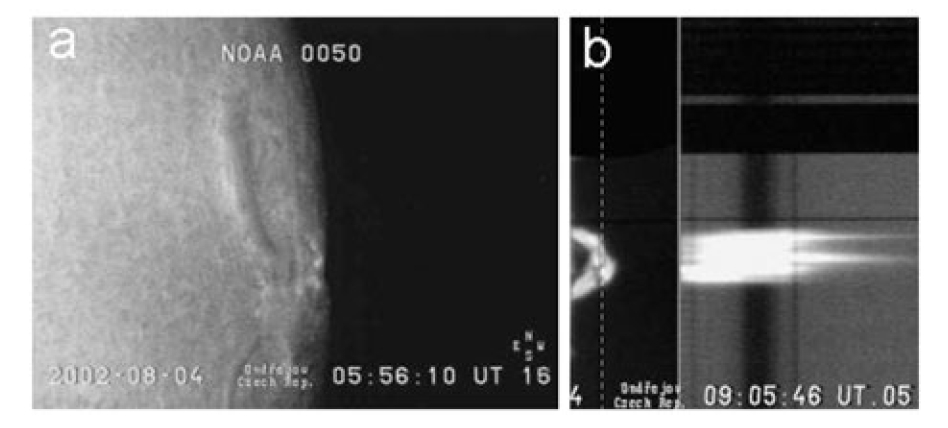
\includegraphics[width=2.5in]{figure2fromHalpha.jpg}
\caption{Observation of a limb event above the sun's surface. $H\alpha$ slit-jaw is the middle (b) part, taken from \cite{miraClanek}.}
\label{figure:observation}
\end{figure}

\subsection{Numerical simulation of magnetohydrodynamics}
From the numerical perspective, to investigate such phenomena is to bring the complexity of multiple scales present in the physical world - magnetic reconnection occurs at substantially different scales than e.g. the solar flares. To handle this numerically with adequate resolution, and reasonable computational costs, the implementation must be able to limit the number of degrees of freedom used for the discretization to such that yield the largest accuracy increase - namely, in this work, this is achieved via a state-of-the-art Adaptive Mesh Refinement approach.
\subsection{Aim of this work}
Main goal that was set for this work is implementation of a software package, capable of numerically solving the magnetohydrodynamic equations with the following attributes:
\begin{itemize}
	\item The code must implement mathematically correct and clean methods, preferably with no parameter-dependent algorithms
	\item The code must allow for a broad spectrum of solution attributes occurring (shocks, oscillations, high energies, ...)
	\item The code must be able to capture very fine details of the solution through higher resolution, in reasonable computing time
	\item The code must be able to run a large-scale simulations, for which a single computer is not sufficient, and utilization of modern distributed computing approach is a must
	\item The code must be easy to use for the physicists, must be written using industry-standard modern object-oriented programming language
\end{itemize}
\subsection{Discontinuous Galerkin method}
We look at the Discontinuous Galerkin method (DG) - which was chosen in order to deliver the first and second of the above requirement (handling sharp fronts, discontinuities and the like with mathematical cleanliness), and give the entire process from the integral equations down to algorithms performing basic operations. Pitfalls of the numerical solution of the MHD equations (divergence constraint, slope limiting), and chosen way of solving them is given as well, while still keeping the above requirements in mind.
\subsection{Automatic Mesh Refinement}
Since the biggest challenge is the satisfaction of the requirement of both the fine resolution of the solution, and the capability of running large-scale simulations on modern distributed computing architecture - while still providing all the other attributes of the implemented code. The approach to this, which involves mainly the Adaptive Mesh Refinement technique (AMR) together with Domain Decomposition technique, is presented and implemented. And finally the verifications, and benchmarks and actual usage on an astrophysical problem are presented.

\section{Discontinuous Galerkin Method}
We start with the ideal MHD equations in the conservative form
\be
\label{conservativeGeneric} \pds{\mrPsi}{t} + \nabla \cdot \mrF\lo\mrPsi\ro = \mrS,
\ee
where we have
\begin{align}
\nonumber
\mrF_i & =  \lo\begin{array}{c} \pi_i \\ \frac{\pi_1 \pi_i}{\rho} - B_1 B_i + \frac12 \delta_{1i} \lo p + U_m\ro \\ \frac{\pi_2 \pi_i}{\rho} - B_1 B_i + \frac12 \delta_{2i} \lo p + U_m\ro \\ \frac{\pi_3 \pi_i}{\rho} - B_1 B_i + \frac12 \delta_{3i} \lo p + U_m\ro \\ \frac{\pi_i}{\rho} \lo \frac{\gamma}{\gamma - 1} p + U_k\ro + \frac{2}{\rho} \varepsilon_{ijk} \lo \pi_k B_i - \pi_i B_k\ro B_j  \\ \frac{\pi_i B_1 - \pi_1 B_i}{\rho}  \\ \frac{\pi_i B_2 - \pi_2 B_i}{\rho} \\ \frac{\pi_i B_3 - \pi_3 B_i}{\rho} \\ \end{array}\ro,\\
\mrPsi & =  \lo\begin{array}{c}\rho \\ \pi_1 \\ \pi_2 \\ \pi_3 \\ U \\ B_1 \\ B_2 \\ B_3 \\ \end{array}\ro,\ 
\mrS =  \lo\begin{array}{c}0 \\ \rho g_1 \\ \rho g_2 \\ \rho g_3 \\ \bfpi \cdot \bfg \\ 0 \\ 0 \\ 0 \\ \end{array}\ro,
\end{align}
where $\varepsilon_{ijk}$ is the Levi-Civita symbol, and $\delta_{ij}$ the Kronecker delta.
\subsection{Weak formulation}
Weak formulation reads
\be
\label{WeakFinal} \int_{\Omega_{t}} \pds{\mrPsi}{t} \mrv - \int_{\Omega_{t}}\mrF\lo\mrPsi\ro \lo\nabla \cdot \mrv\ro + \int_{\partial\Omega_{t}} \lo\mrF\lo\mrPsi\ro \cdot \bfn \ro\mrv = \int_{\Omega_{t}} \mrS \mrv,
\ee
where the terms $\mrF\lo\mrPsi\ro \lo\nabla \cdot \mrv\ro; \lo\mrF\lo\mrPsi\ro \cdot \bfn \ro\mrv$ are meant as a component-wise multiplication, $\Omega_t$ is a domain occupied by the fluid at time $t$, and $\mrv$ are test functions from a suitable Sobolev space.
\subsection{Discretization}
We employ the standard \textit{broken Sobolev space}, obtaining thus a finite dimensional space of basis\/test functions defined on hexahedral elements. Since we are interested in large scale problems, the domain is decomposed using standard approaches to do so - using the MPI communication layer implemented in the deal.II and Trilinos frameworks.
\begin{figure}[!t]
		\begin{center}
			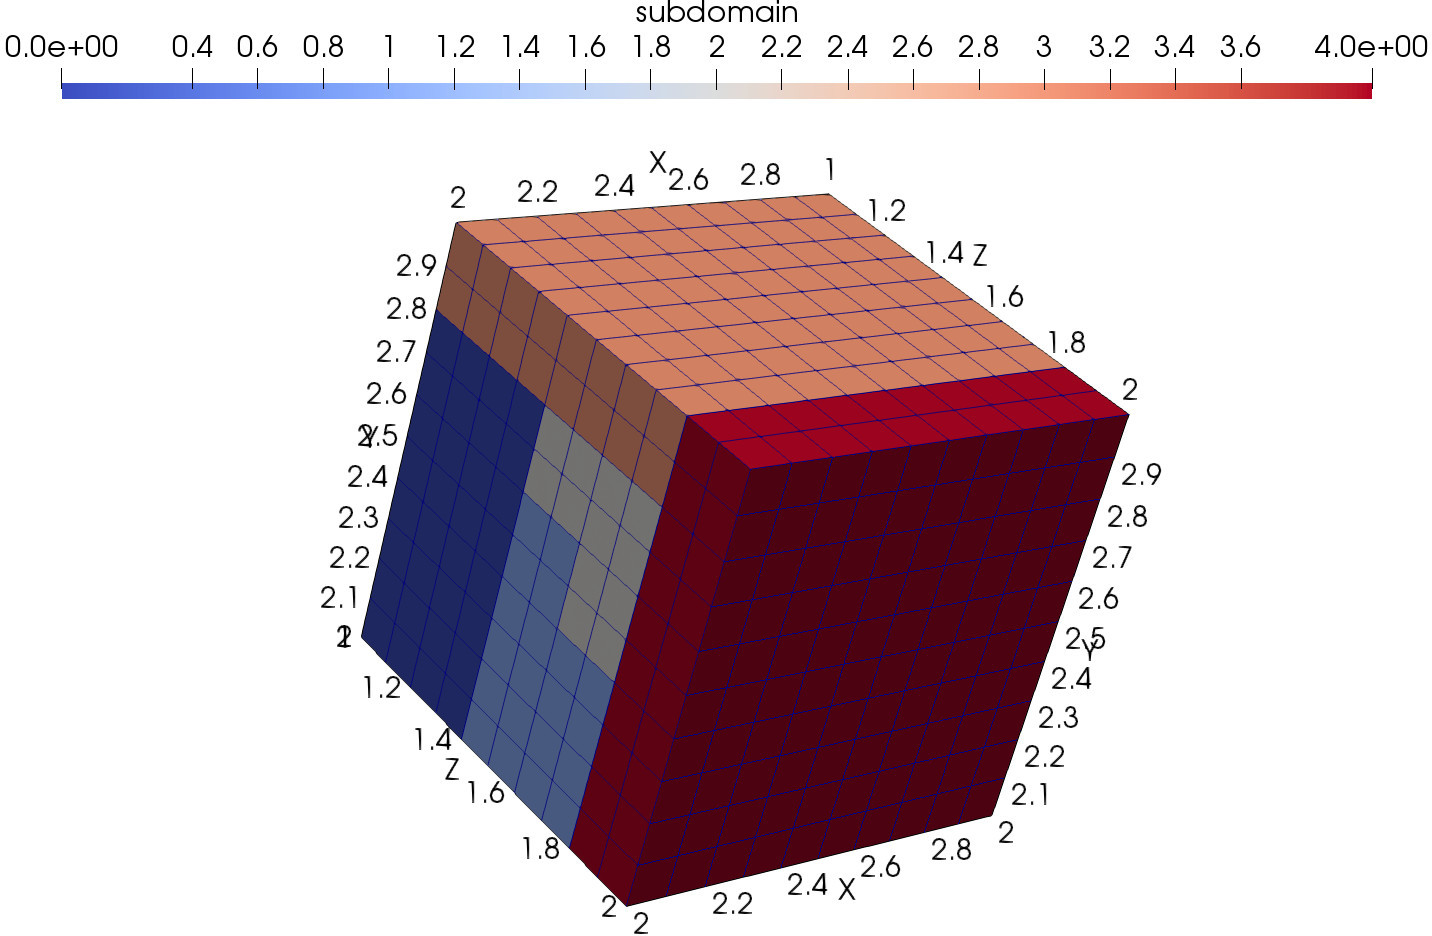
\includegraphics[width=2.5in]{cube.jpg}
		\caption{Cubical domain $\Omega$ with color-coded processor-owned elements.}
		\label{figure:domainDecomposition}
		\end{center}
	\end{figure}\vspace{-5mm}
	
\subsection{Divergence-free FE space}
The divergence-free constraint of the magnetic field, $\nabla \cdot \bfB = 0$ (Gauss's law) is not enforced by the solution of the problem \ref{WeakFinal}. Therefore, we need to perform additional work to be sure that we do not have a non-physical solution in the sense that the constraint is not satisfied.
There are two often used approaches to handle this problem - the Constraint-Transport (CT) method, and divergence cleaning. The first one is not suitable for this work, as it constraints the triangulation in such a way, that implementing Adaptive Mesh Refinement would be very complicated, if possible at all. The second approach, the divergence cleaning methods need additional postprocessing step which may be omitted for the sake of calculation efficiency.
The approach taken in this work is to replace the standard FE space with such basis functions for the magnetic field component ($B$) with a vector-valued (3-dimensional) space $V_h^B$ of functions that have exactly
\be
\nabla \cdot \mrvh^B = 0,\ \ \mrvh^B\in V_h^B,
\ee
where these functions are as before discontinuous on element interfaces $\Gamma_{ij}$. An example of such a function is in Figure \ref{figure:divFree}
\begin{figure}[!t]
		\begin{center}
			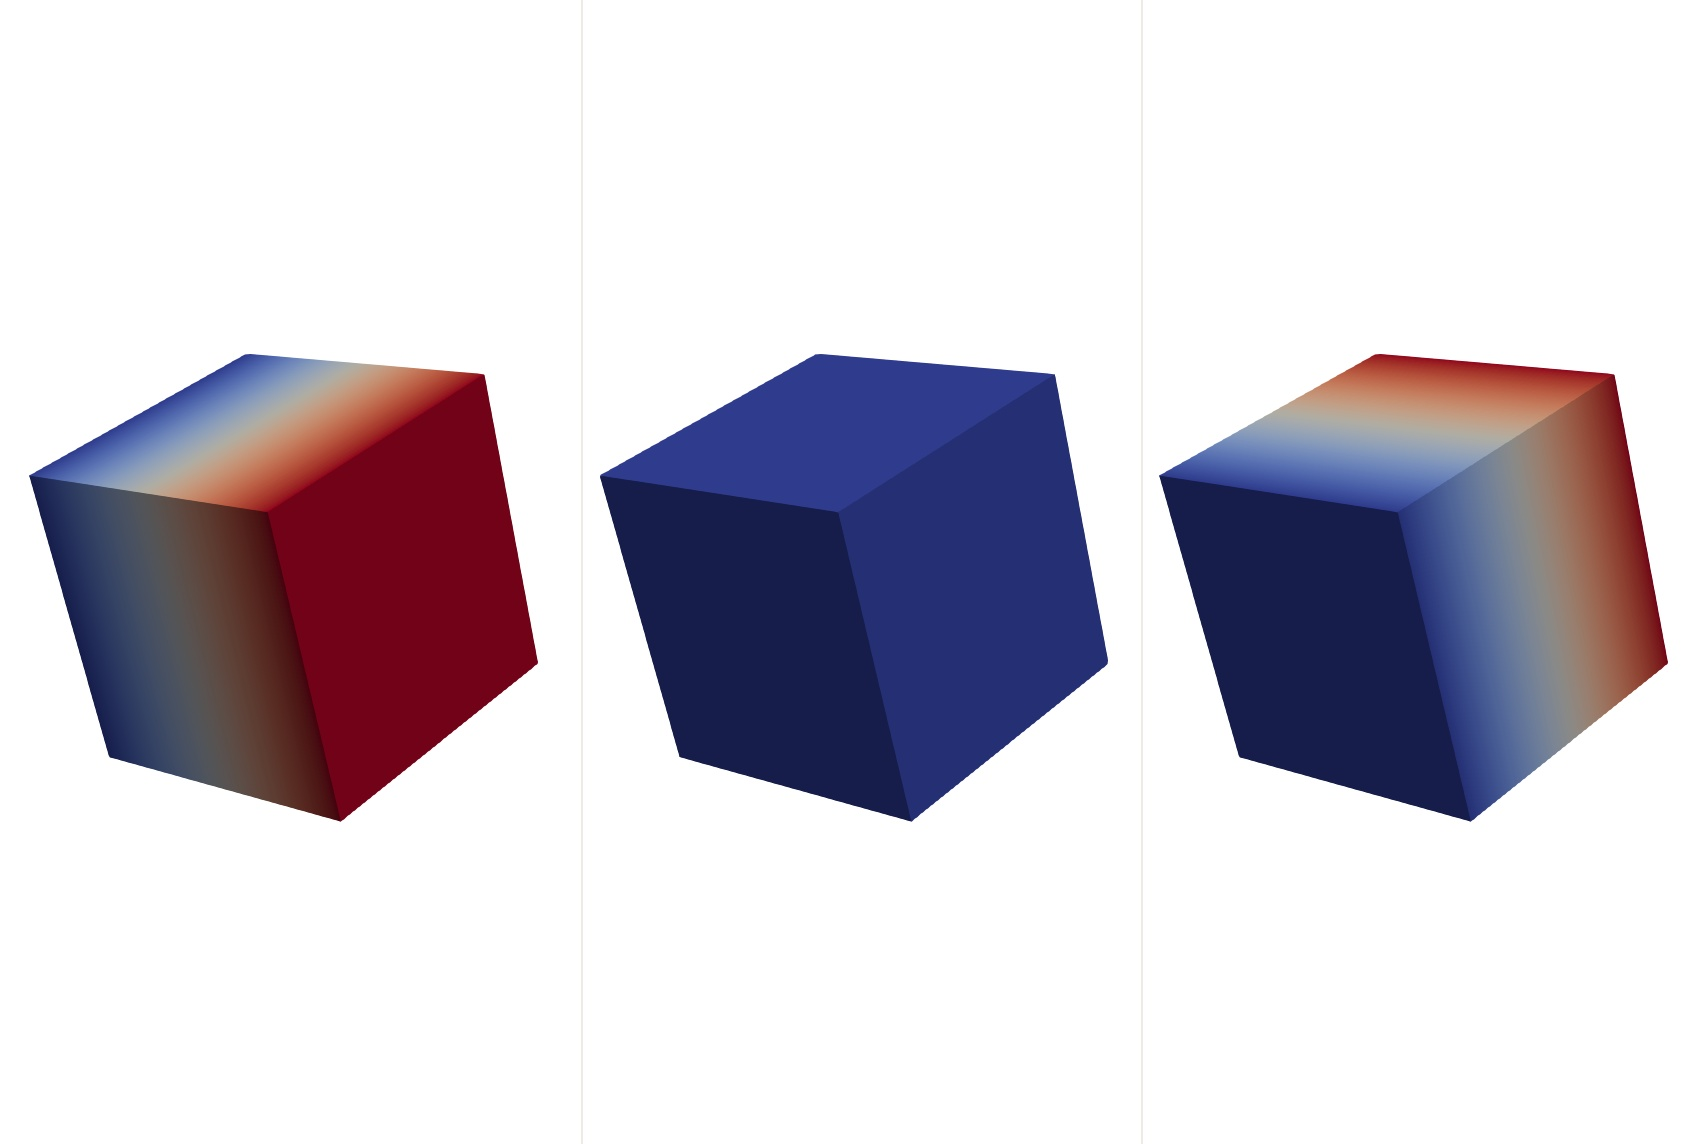
\includegraphics[width=2.5in]{divFree.jpg}
		\caption{One of the divergence-free basis functions.}
		\label{figure:divFree}
		\end{center}
	\end{figure}\vspace{-5mm}
	
\subsection{Slope limiting}
It is well known that the Discontinuous Galerkin method exhibits nonphysical spurious oscillations in the vicinity of sharp discontinuities. Noteworthy is the fact, that with continuous Finite Element spaces, the situation is even worse, as the oscillations tend to propagate through the computational domain. With the DG method, the problem is localized to a single layer of elements bordering any sharp front. This behavior is not acceptable, and measures must be taken to eliminate such oscillations - methods aiming at solving this are usually labeled as flux limiters, slope limiters, or shock capturing schemes.
\subsubsection*{}
These methods can be categorized according to multiple aspects. Out of these, two are important from the perspective of this work. First categorization is whether the approach changes the equations by introducing additional term that 'smoothes' the solution near the sharp front (this may be understood as a form of \textit{artificial viscosity / resistivity}). In this work, such an approach is not preferred, as we aim at implementing a generally usable solver, where extensive analysis of the impact of a change in the governing equations for the particular problem is not possible.

\subsubsection{Vertex-based limiter}
Introduced by D. Kuzmin in \cite{KuzminVertex}, the Vertex-based limiter aims at being an improvement over the Barth-Jespersen limiter. It considers the solution in the form
\be
\label{slopeLimSln}
u_h\lo x\ro = u_c + \alpha_e\lo\nabla u\ro_c \cdot \lo x - x_c\ro,\ 0 \leq \alpha_e\leq 1,
\ee
but the definition of the correction factor $\alpha_K$ reads

\be
\label{vertexBasedAlpha}
\alpha_K = \min_i\left\{\begin{array}{c}
\min\left\{1, \frac{u_i^{max} - u_c}{u_i - u_c}\right\},\ if\ \ u_i - u_c > 0,\\
1,\ \ \ \ \  \  \  \  if\ u_i - u_c = 0,\\
\min\left\{1, \frac{u_i^{min} - u_c}{u_i - u_c}\right\},\ if\ \ u_i - u_c < 0,\end{array}\right.
\ee
where in this case $u_i^{min}, u_i^{min}$ are defined in such a way that for each of the vertices they are initialized with a small and a large constant, respectively, and then in the loop over all elements that contain the $i-$th vertex, the values are updated as:
\be
u_i^{max} = \max\left\{u_c, u_i^{max}\right\},\ \ u_i^{min} = \min\left\{u_c, u_i^{min}\right\}.
\ee
This slope limiting technique proves to have all the required attributes from the perspective of this work.
A comparison between an unlimited (\ref{figure:unlimited}) and limited (\ref{figure:limited}) solution is given in figures in this section.
\begin{figure}[!t]
		\begin{center}
			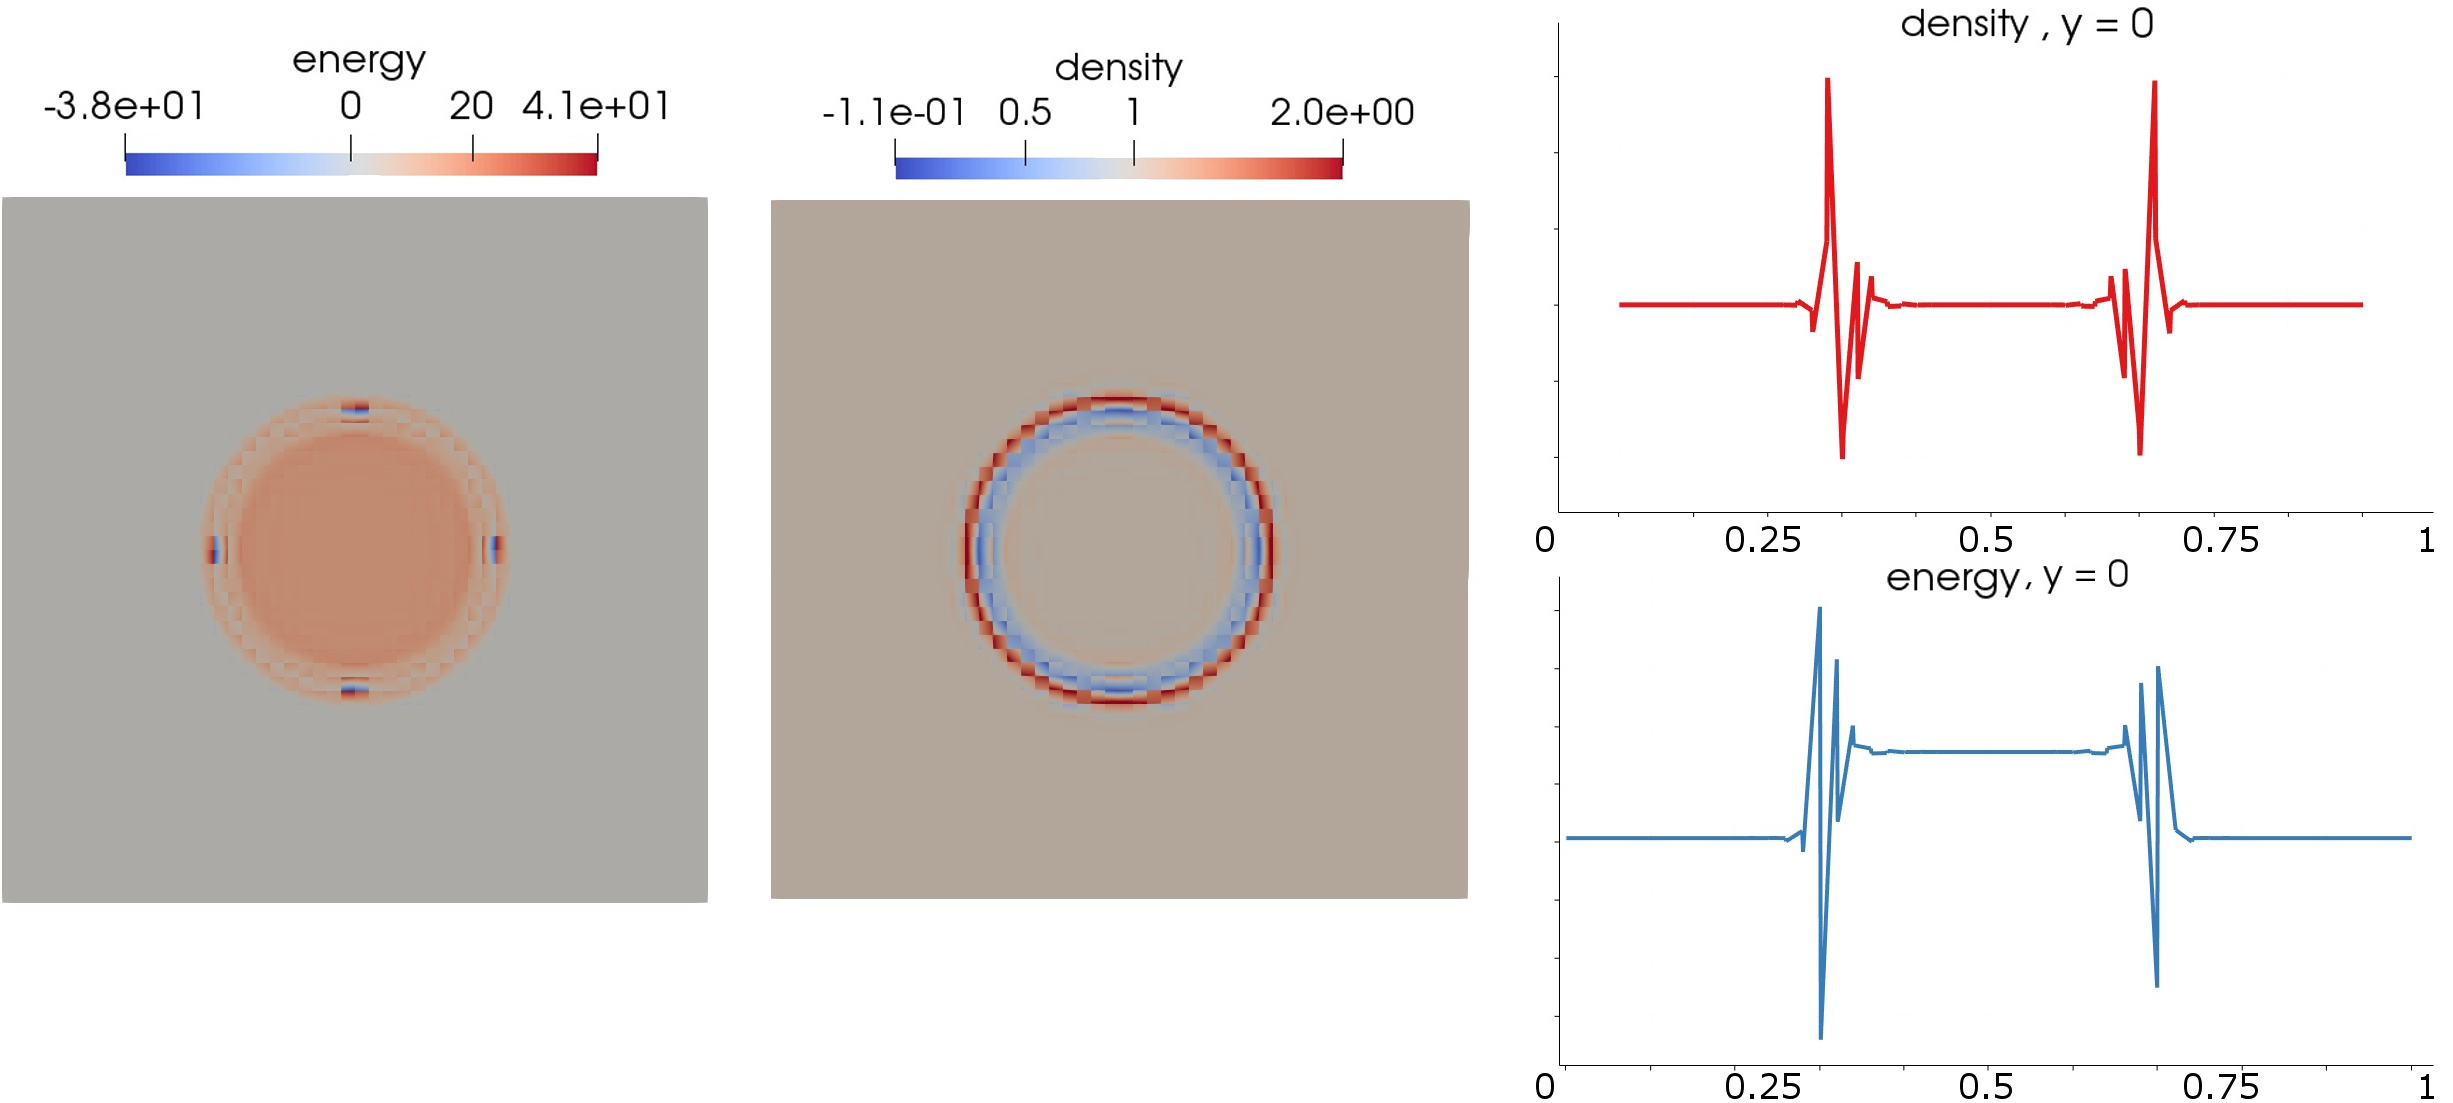
\includegraphics[width=2.5in]{nl6.jpg}
		\caption{Unlimited solution.}
		\label{figure:unlimited}
		\end{center}
	\end{figure}
	
\begin{figure}[!t]
		\begin{center}
			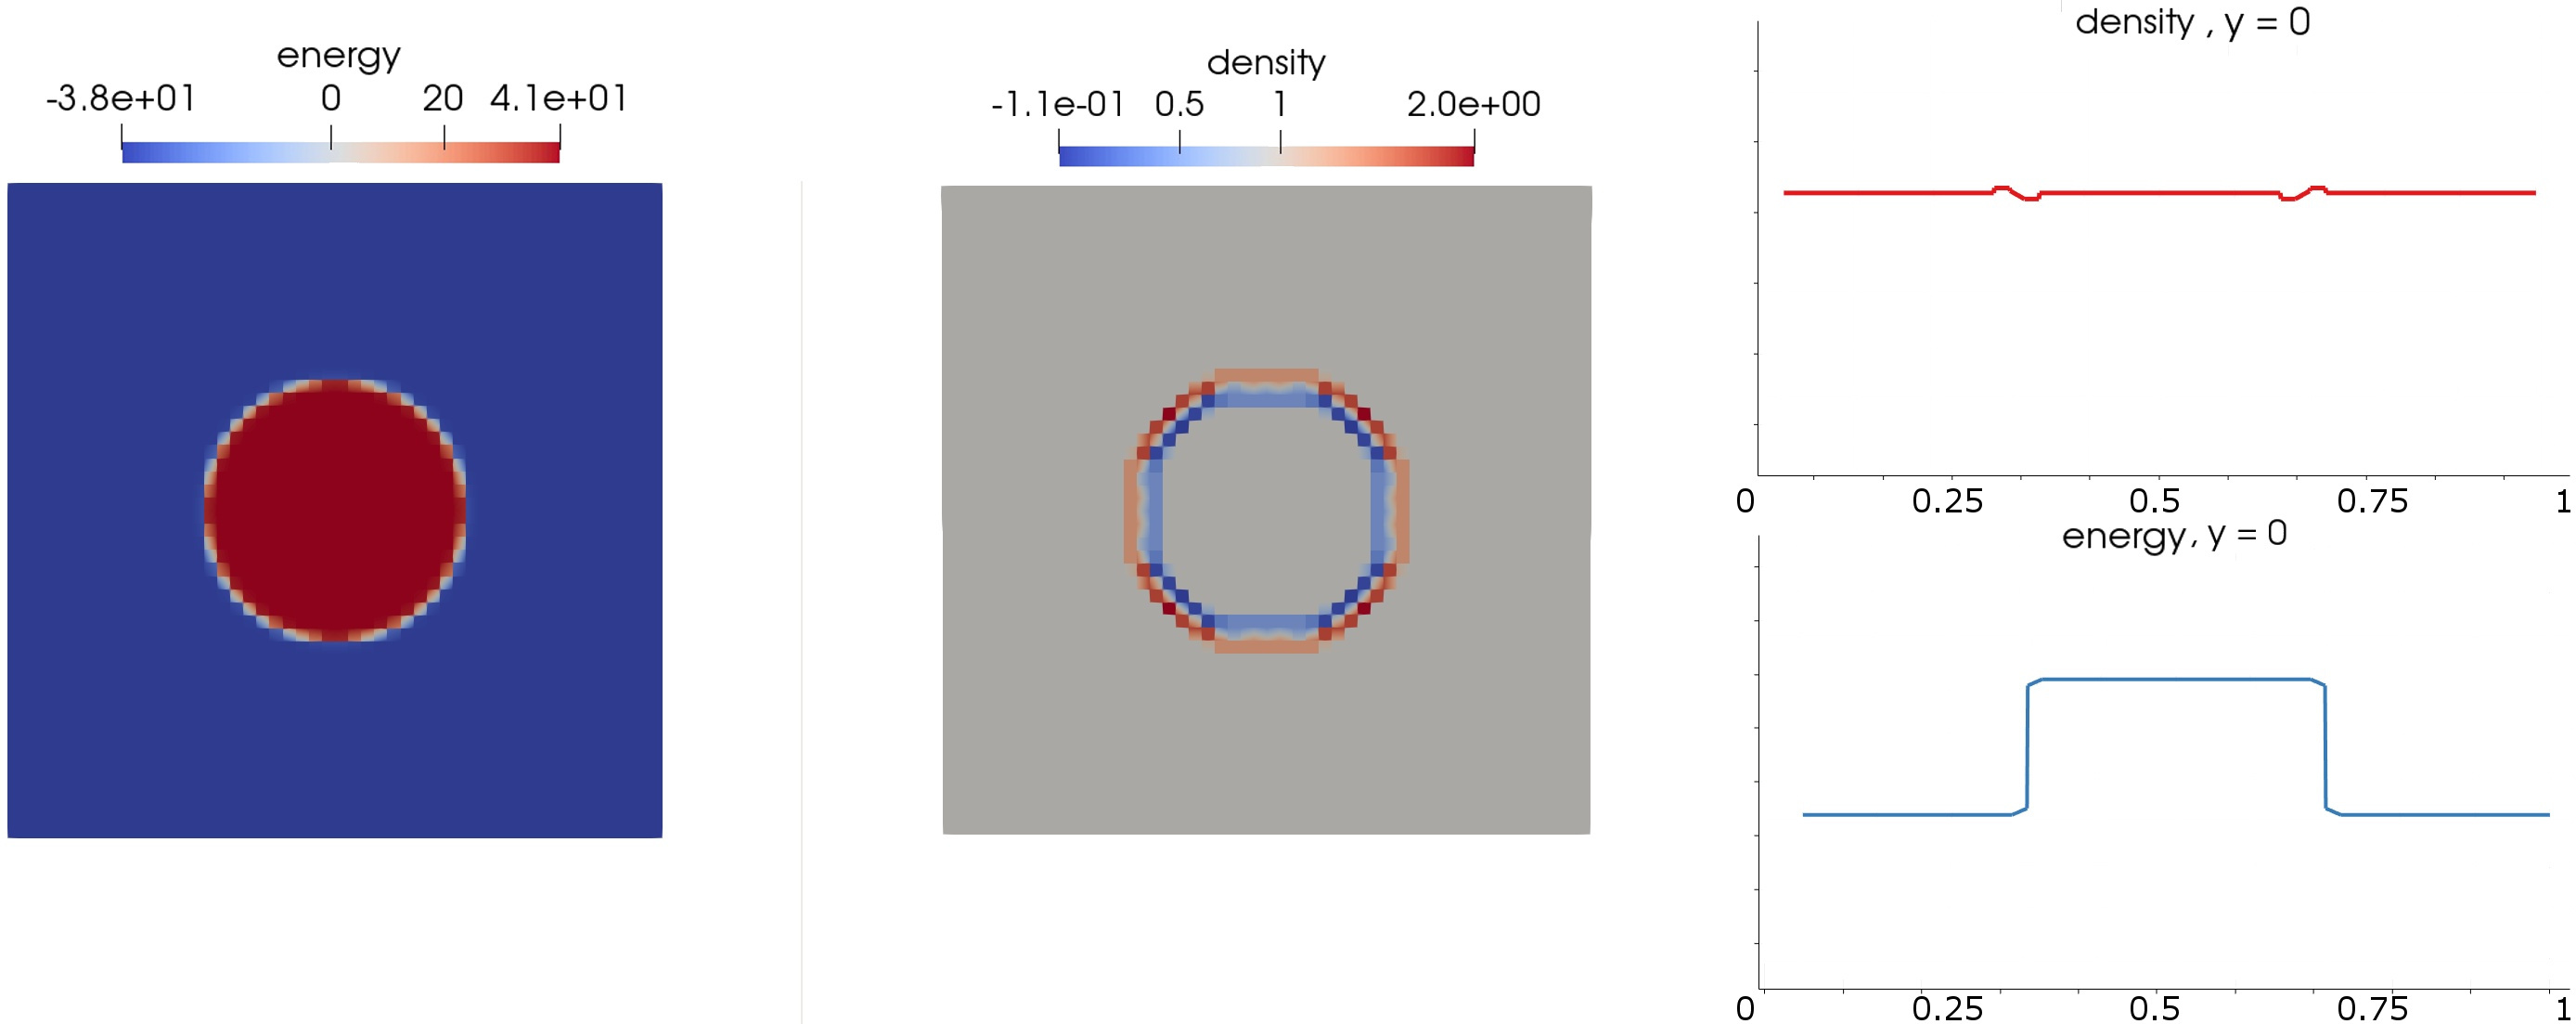
\includegraphics[width=2.5in]{l1.jpg}
		\caption{Limited solution.}
		\label{figure:limited}
		\end{center}
	\end{figure}
	
\section{Automatic Mesh Refinement}
As the Adaptive Mesh Refinement (AMR) is a very important algorithm in the overall numerical solution, handling the multi-scale aspect of the studied problems, in this chapter, a description of what needs to be taken care of for the DG method, in the distributed settings, and what concrete decisions were made during this work, and justification of these in light of the requirements on the numerical solution.
The general schema of any Adaptive Mesh Refinement algorithm is described in the algorithm \ref{algorithm:AMRGen}:
\ \\
\begin{algorithm}
 \KwData{Mesh $T_0$}
 \KwResult{A mesh $T_n$ and a solution $\bfy_n$ on this mesh satisfying the solution acceptance criteria}
 i = 0\\
 \While{true}{
  obtain solution $\bfy_i$ on $T_i$\\
	evaluate solution $\bfy_i$ acceptance criteria\\
	\eIf{solution acceptance criteria satisfied} {
		return\\
   } {
		identify subset $T^{r}_i$ of all elements $K \in T_i$ to be refined, $T^{r}_i \subseteq T_i$\\
		obtain $T_{i+1}$ by refining (at least) all $K \in T^{r}_i$\\
		i = i + 1\\
	}
 }
 \caption{Generic AMR algorithm}
\label{algorithm:AMRGen}
\end{algorithm}
In \ref{algorithm:AMRGen}, \textit{solution acceptance criteria} is usually either spatial error estimate threshold, or number of elements, etc.

\section{Results}
Several benchmarks (MHD Blast, Orszag-Tang vortex) - \ref{figure:blastFinal}, \ref{figure:ot}, as well as a simulation of a flux-rope based on Titov-Demoulin model (\ref{figure:td}) have been done.
\begin{figure}
	\begin{center}
		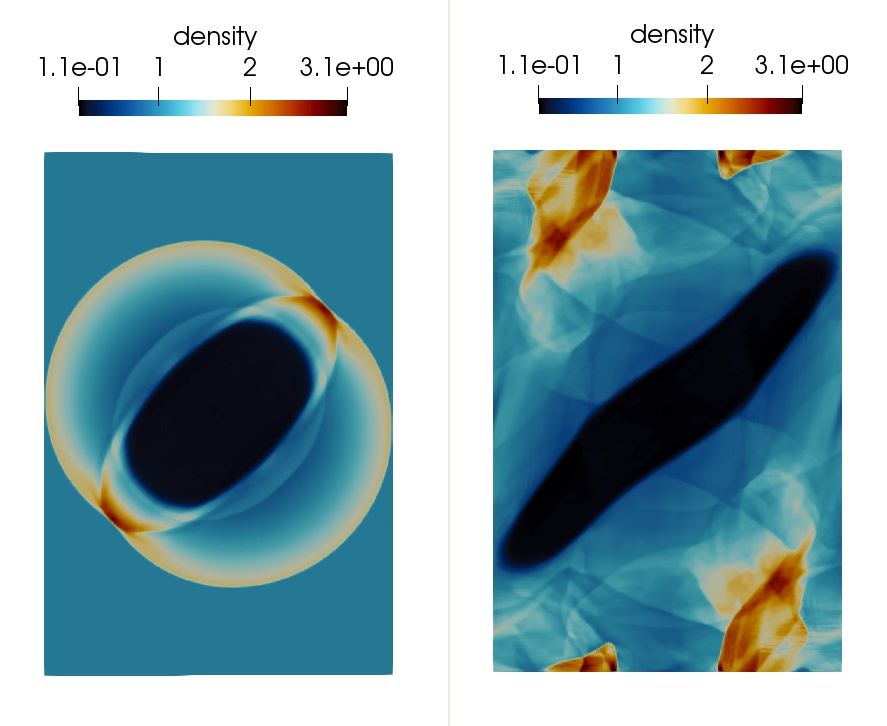
\includegraphics[width=2.5in]{ref-result.jpg}
	\caption{MHD Blast problem, obtained $\rho$ distribution, $t \approx 0.2$ (left), $t \approx 1.0$ (right).}
	\label{figure:blastFinal}
	\end{center}
\end{figure}
\begin{figure}
	\begin{center}
		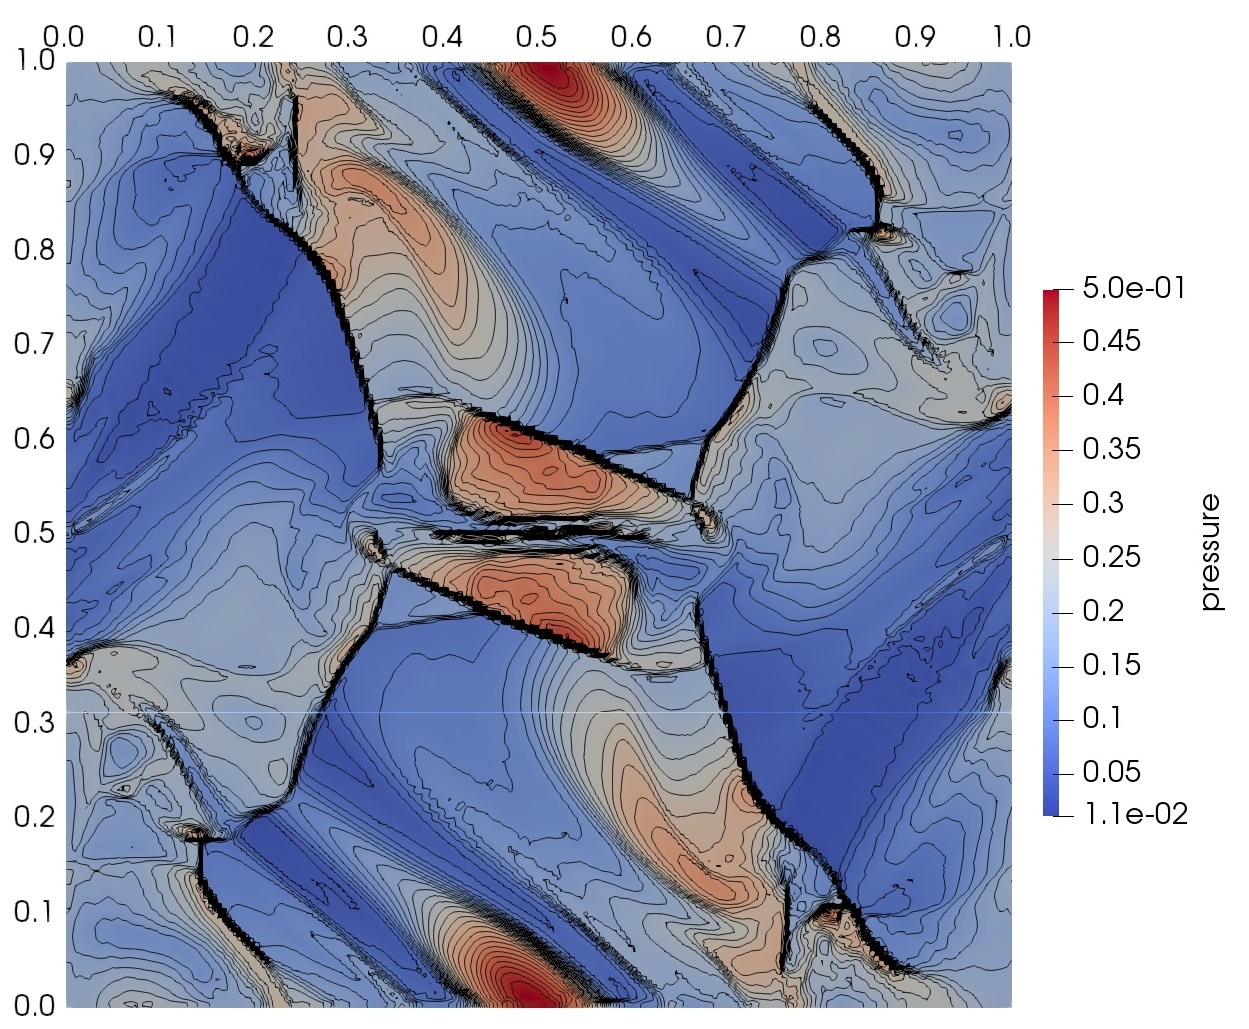
\includegraphics[width=2.5in]{ot.jpg}
	\caption{Orszag-Tang problem, obtained $p$ distribution at time $t \approx 0.5$.}
	\label{figure:ot}
	\end{center}
\end{figure}

\begin{figure}
	\begin{center}
		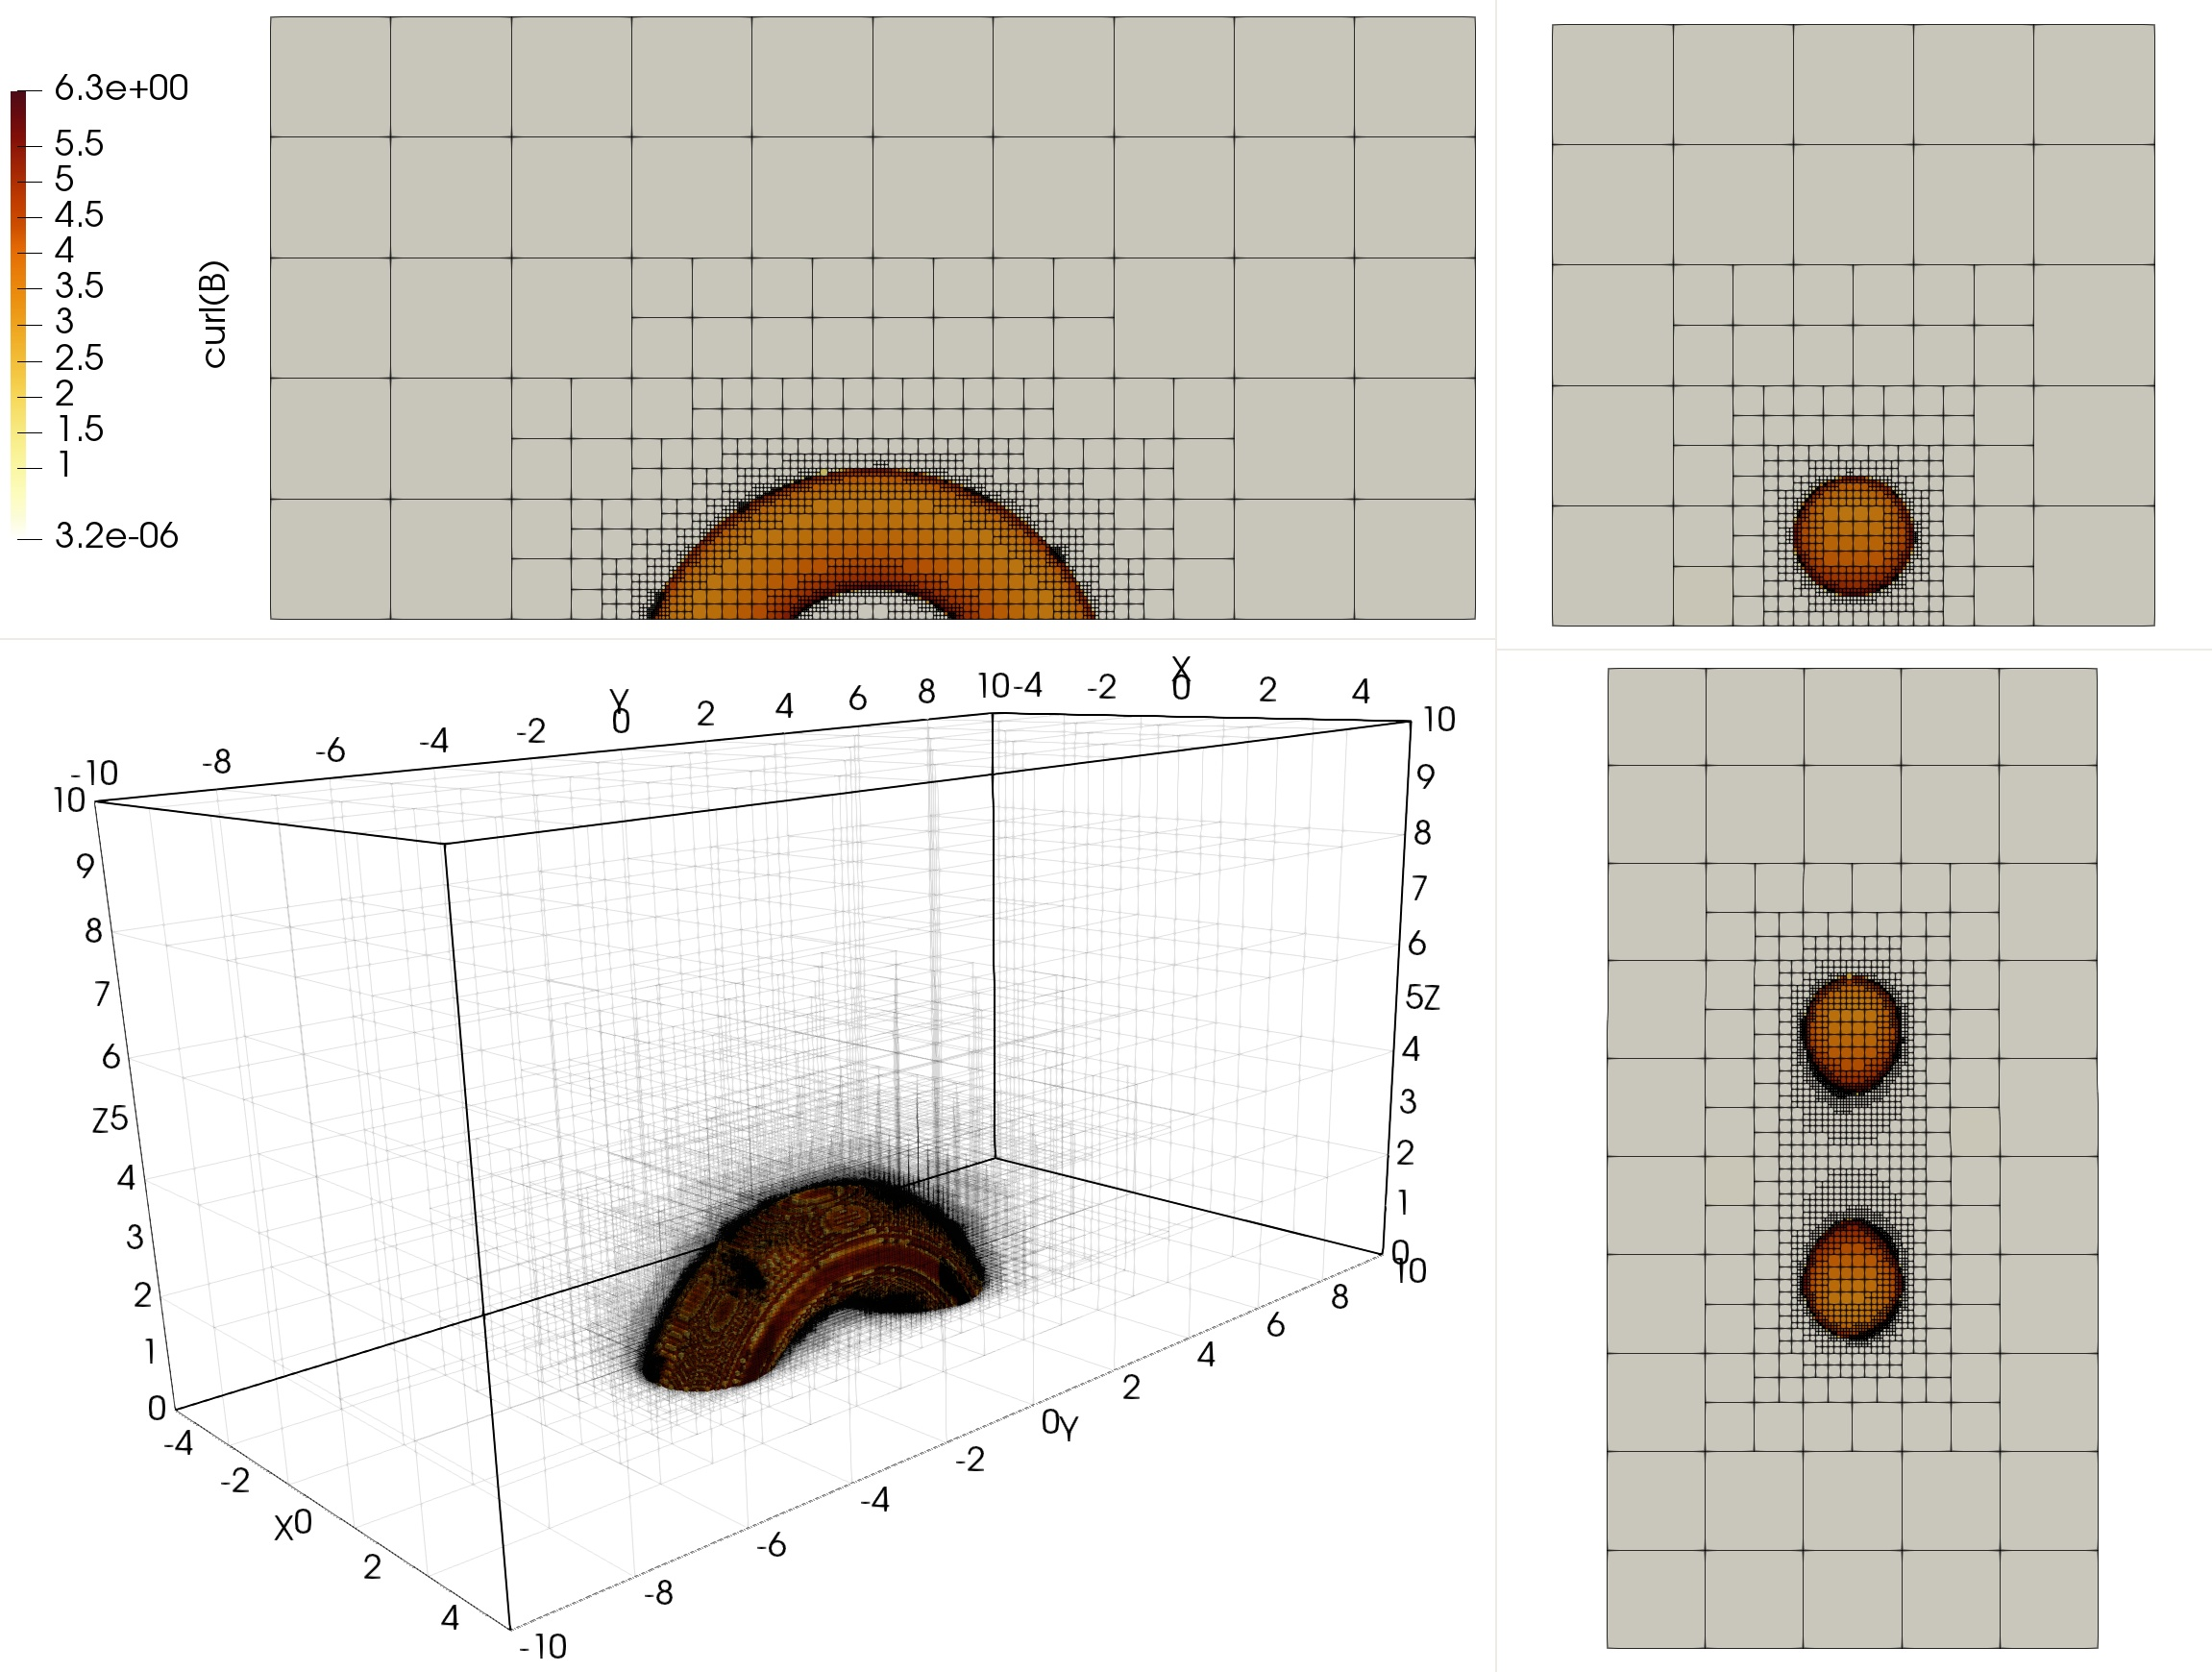
\includegraphics[width=2.5in]{td6.jpg}
	\caption{Titov-Demoulin model, AMR result.}
	\label{figure:td}
	\end{center}
\end{figure}



\section{Conclusion}
The goal of this work has been accomplished, and a software package implementing the discontinuous Galerkin method for MHD equations, together with AMR functionality, and without presence of artificial parameters in the implemented algorithms, was implemented. Further work in employing the software for solution of MHD problems in astrophysics is being done.

% use section* for acknowledgment
\section*{Acknowledgment}
The authors would like to thank...


% Can use something like this to put references on a page
% by themselves when using endfloat and the captionsoff option.
\ifCLASSOPTIONcaptionsoff
  \newpage
\fi

% references section
% can use a bibliography generated by BibTeX as a .bbl file
% BibTeX documentation can be easily obtained at:
% http://mirror.ctan.org/biblio/bibtex/contrib/doc/
% The IEEEtran BibTeX style support page is at:
% http://www.michaelshell.org/tex/ieeetran/bibtex/
%\bibliographystyle{IEEEtran}
% argument is your BibTeX string definitions and bibliography database(s)
%\bibliography{IEEEabrv,../bib/paper}
%
% <OR> manually copy in the resultant .bbl file
% set second argument of \begin to the number of references
% (used to reserve space for the reference number labels box)
\bibliographystyle{ieeetran}
\bibliography{8-bibliography}

\begin{IEEEbiographynophoto}{Lukas Korous}
Biography text here.
\end{IEEEbiographynophoto}

\begin{IEEEbiographynophoto}{Pavel Karban}
Biography text here.
\end{IEEEbiographynophoto}

\end{document}


